\documentclass[11pt]{article}
\usepackage[utf8]{inputenc}
\usepackage[T1]{fontenc}
\usepackage{geometry}
\geometry{letterpaper,margin=1in}
\usepackage{booktabs}
\usepackage{amsmath}
\usepackage{amssymb}
\usepackage{graphicx}
\usepackage{hyperref}
\usepackage{natbib}
\usepackage{enumitem}
\usepackage{tikz}
\usetikzlibrary{arrows.meta,positioning,shapes.geometric,fit,calc}

\title{SHARD: Composable Infrastructure for Self-Healing, Persistent LLM Agents}
\author{Christopher Aytona}
\date{}

\begin{document}
\maketitle

\begin{abstract}
Large language model agents deployed in persistent, multi-session environments face compounding challenges: memory degrades without governance, coordination between concurrent agents lacks formal guarantees, skill acquisition proceeds without quality control, and self-improvement operates without safety bounds. We present SHARD (Self-Healing Agent with Resilient Delegation), a harness-agnostic application architecture that composes four independent subsystems---memory governance with staleness detection, intent-based coordination protocol, quality-gated skill lifecycle with trust tiers, and safety-constrained self-improvement---into an integrated infrastructure where emergent behaviors arise from their interaction. Our contribution is the architecture and its composition properties. We validate the design through targeted mechanism tests that demonstrate composition produces capabilities none of the subsystems could achieve independently, and we report both successes and identified design gaps with equal transparency.
\end{abstract}

\section{Introduction}

The deployment of LLM-based agents beyond single-session interactions introduces failure modes absent from conversational AI research. An agent that persists across hundreds of sessions accumulates stale knowledge, spawns concurrent workers without coordination guarantees, acquires capabilities without vetting, and modifies its own configuration without understanding downstream consequences. These are not independent problems---they interact multiplicatively. Stale memory corrupts coordination decisions. Unvetted skills introduce unsafe self-modification paths. Uncoordinated agents duplicate work or produce conflicting state changes.

Existing frameworks address subsets of these challenges in isolation. MemGPT \citep{packer2023memgpt} introduces hierarchical memory but lacks coordination primitives. AutoGen \citep{wu2023autogen} provides multi-agent conversation but without persistent memory or self-improvement governance. Voyager \citep{wang2023voyager} demonstrates skill acquisition but without trust tiers or safety bounds. No existing system addresses the \emph{composition} of these concerns---the interactions between memory, coordination, governance, and safety that dominate real-world persistent deployments.

We present SHARD, built on a production LLM agent harness. Where the harness provides the substrate---session management, tool connectivity, basic scheduling, and subagent spawning---SHARD contributes the architectural layer that makes persistent autonomous operation viable. Our contribution is not any single subsystem but their \emph{composition}: the demonstration that four independently-motivated components, when designed with explicit composition interfaces, produce emergent behaviors that address the multiplicative failure modes of persistent agents.

\section{Background: The Harness Substrate}

SHARD is built atop an LLM agent harness---a persistent runtime layer that manages one or more LLM-backed agents, providing session lifecycle, tool dispatch, memory persistence, scheduling, multi-agent coordination, and fault recovery, independent of the underlying model. Examples of such harnesses include OpenClaw, Claude Code (Anthropic), Hermes Agent (NousResearch), AutoGen (Microsoft), CrewAI, LangGraph (LangChain), Semantic Kernel (Microsoft), and similar MCP-compatible runtimes that provide session management, tool connectivity, and basic scheduling primitives. We use one such harness as our substrate. Understanding what the harness provides---and critically, what it lacks---motivates SHARD's design.

\subsection{Harness Capabilities}

The harness provides six core primitives. First, a \emph{harness process} manages LLM sessions, routing user messages from Slack or a web dashboard to an underlying language model with tool-use capabilities. Second, \emph{MCP (Model Context Protocol) connections} expose external tools---databases, APIs, file systems---as callable functions within agent sessions. Third, \emph{cron scheduling} enables recurring or one-shot jobs that spawn independent agent sessions on a timer. Fourth, \emph{subagent spawning} allows a running session to delegate tasks to parallel worker sessions, receiving results asynchronously. Fifth, \emph{persistent memory} stores user preferences, project context, daily history, semantic key-value pairs, and learned corrections across sessions---providing raw storage that survives session boundaries. Sixth, a \emph{skill system} loads markdown instruction files that shape agent behavior for specific domains.

\subsection{Harness Gaps}

Four critical gaps emerge when harness-based agents operate persistently across hundreds of sessions over weeks or months.

\textbf{Persistence without governance.} Memory storage exists but lacks intelligence. Entries accumulate without staleness detection, conflict resolution, or hierarchical organization. A correction from day one carries equal weight to one from yesterday, even when the underlying system has changed. No mechanism distinguishes between facts that decay (API endpoints, team structures) and invariants that persist (coding conventions, safety rules). No process detects when two memory entries contradict each other.

\textbf{Coordination without guarantees.} Subagent spawning is fire-and-forget. No protocol prevents two agents from modifying the same file, no mechanism declares intent before action, and no review phase catches conflicts before execution. The parent session receives results but cannot reason about inter-agent dependencies.

\textbf{Capability acquisition without vetting.} Skills (markdown instruction files) can be added to the agent's repertoire without quality assessment, trust classification, or graduated deployment. A skill imported from an external marketplace receives the same authority as one battle-tested over months of production use.

\textbf{Self-modification without bounds.} The agent can modify its own configuration, create new cron jobs, alter skill files, and restructure memory---but no mechanism constrains \emph{what} it may modify, \emph{how much} it may change in a single operation, or \emph{whether} a modification is reversible.

\section{SHARD Architecture}

SHARD addresses each gap through a dedicated subsystem, designed with explicit \emph{composition interfaces} that enable cross-subsystem interaction (Figure~\ref{fig:architecture}). We define a composition interface as a typed read/write protocol between subsystems: each subsystem exposes specific state (memory entries, trust scores, staleness signals, safety verdicts) through well-defined queries, and consumes state from others through the same mechanism. These interfaces are not implementation-specific---they define \emph{what} information flows between subsystems, not how it is stored or transmitted.

\begin{figure}[ht]
\centering
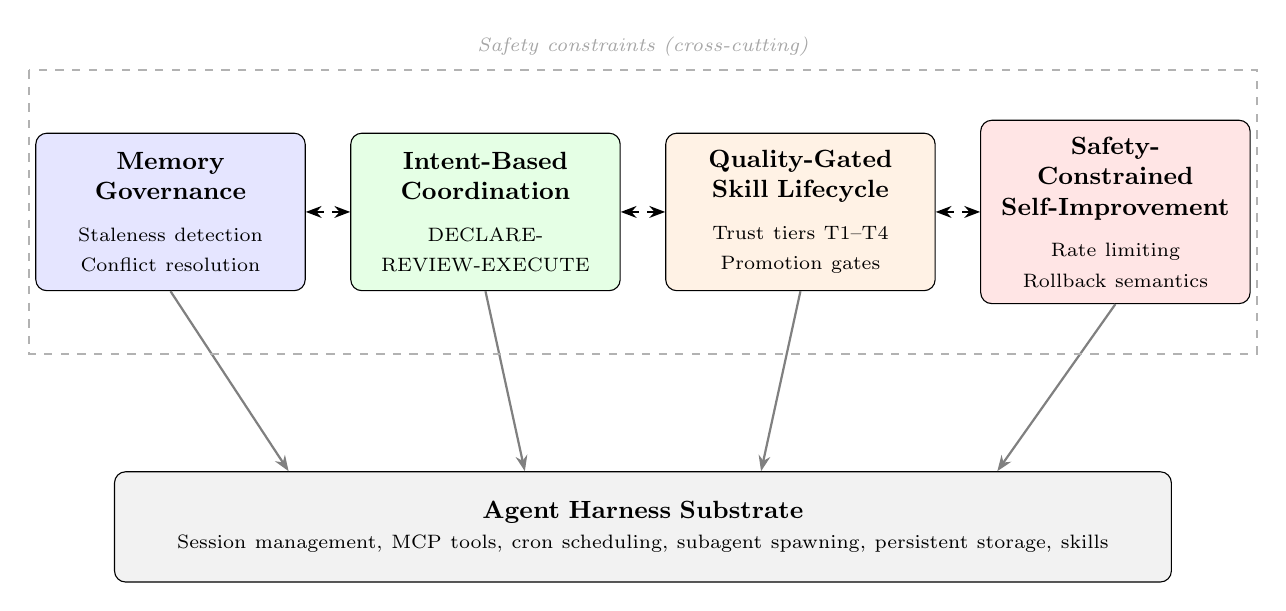
\begin{tikzpicture}[
    box/.style={draw, rounded corners, text width=3cm, minimum height=2cm, align=center, font=\small, inner sep=6pt},
    substrate/.style={draw, fill=gray!10, rounded corners, text width=13cm, minimum height=1.4cm, align=center, font=\small, inner sep=6pt},
    arrow/.style={-{Stealth[length=2mm]}, thick, gray}
]
% Substrate at bottom
\node[substrate] (gw) at (6,-4) {\textbf{Agent Harness Substrate}\\{\scriptsize Session management, MCP tools, cron scheduling, subagent spawning, persistent storage, skills}};

% Four subsystems in a row
\node[box, fill=blue!10] (mem) at (0,0) {\textbf{Memory Governance}\\[4pt]{\scriptsize Staleness detection}\\{\scriptsize Conflict resolution}};
\node[box, fill=green!10] (coord) at (4,0) {\textbf{Intent-Based Coordination}\\[4pt]{\scriptsize DECLARE-REVIEW-EXECUTE}};
\node[box, fill=orange!10] (skill) at (8,0) {\textbf{Quality-Gated Skill Lifecycle}\\[4pt]{\scriptsize Trust tiers T1--T4}\\{\scriptsize Promotion gates}};
\node[box, fill=red!10] (safe) at (12,0) {\textbf{Safety-Constrained Self-Improvement}\\[4pt]{\scriptsize Rate limiting}\\{\scriptsize Rollback semantics}};

% Composition arrows between subsystems
\draw[{Stealth[length=2mm]}-{Stealth[length=2mm]}, thick, dashed] (mem.east) -- (coord.west);
\draw[{Stealth[length=2mm]}-{Stealth[length=2mm]}, thick, dashed] (coord.east) -- (skill.west);
\draw[{Stealth[length=2mm]}-{Stealth[length=2mm]}, thick, dashed] (skill.east) -- (safe.west);

% Down arrows to substrate
\draw[arrow] (mem.south) -- ($(gw.north)+(-4.5,0)$);
\draw[arrow] (coord.south) -- ($(gw.north)+(-1.5,0)$);
\draw[arrow] (skill.south) -- ($(gw.north)+(1.5,0)$);
\draw[arrow] (safe.south) -- ($(gw.north)+(4.5,0)$);

% Safety cross-cutting label
\draw[dashed, thick, gray!60] (-1.8,1.8) rectangle (13.8,-1.8);
\node[font=\scriptsize\itshape, gray!70] at (6,2.1) {Safety constraints (cross-cutting)};
\end{tikzpicture}
\caption{SHARD architecture overview. Four subsystems with composition interfaces (dashed arrows) showing bidirectional data flow. Safety constraints operate as a cross-cutting concern. The agent harness substrate provides runtime primitives.}
\label{fig:architecture}
\end{figure}

\subsection{Memory Governance with Staleness Detection}

\textbf{Problem.} The harness provides persistent memory storage (lessons, preferences, projects, history, semantic key-value pairs) but offers no governance over that storage. Entries accumulate without staleness detection, contradictions go unresolved, and no signal distinguishes fresh facts from outdated beliefs.

\textbf{Design.} SHARD does not replace the harness's memory---it adds a governance layer that classifies, monitors, and maintains the existing storage. SHARD imposes three governance tiers on the harness's flat memory:

\begin{itemize}[nosep]
\item \emph{Semantic memory} stores factual key-value pairs with timestamps, source attribution, and declared decay classes (ephemeral: days, contextual: weeks, durable: months, invariant: permanent).
\item \emph{Episodic memory} retains conversation fragments with relevance scoring and automatic summarization at configurable intervals.
\item \emph{Procedural memory} encodes learned corrections and behavioral rules with conflict detection---new entries are checked against existing rules for contradiction before admission.
\end{itemize}

\textbf{Key Mechanism: Staleness Detection.} Each memory entry carries a \texttt{last\_verified} timestamp and a decay class. A background process computes staleness scores:

\begin{equation}
\text{staleness} = \frac{\text{now} - \text{last\_verified}}{\text{expected\_lifetime}(\text{decay\_class})}
\end{equation}

Entries exceeding a staleness threshold of 1.0 are flagged for re-verification rather than silently served. Entries exceeding 2.0 are quarantined---still retrievable but marked as potentially invalid.

\begin{figure}[ht]
\centering
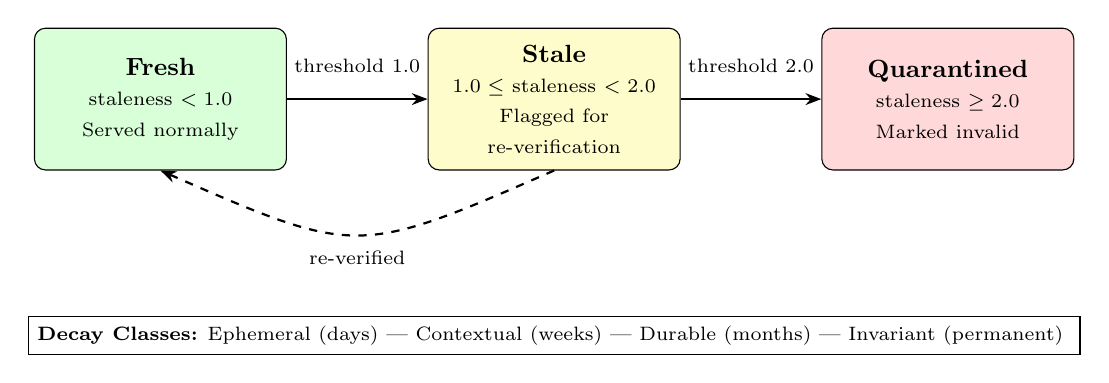
\begin{tikzpicture}[
    zone/.style={draw, minimum width=3.2cm, minimum height=1.8cm, align=center, font=\small, rounded corners},
    arrow/.style={-{Stealth[length=2mm]}, thick}
]
% Zones with more horizontal spacing
\node[zone, fill=green!15] (fresh) at (0,0) {\textbf{Fresh}\\{\scriptsize staleness $< 1.0$}\\{\scriptsize Served normally}};
\node[zone, fill=yellow!20] (stale) at (5,0) {\textbf{Stale}\\{\scriptsize $1.0 \leq$ staleness $< 2.0$}\\{\scriptsize Flagged for}\\{\scriptsize re-verification}};
\node[zone, fill=red!15] (quar) at (10,0) {\textbf{Quarantined}\\{\scriptsize staleness $\geq 2.0$}\\{\scriptsize Marked invalid}};

% Arrows with labels well above
\draw[arrow] (fresh.east) -- (stale.west) node[midway, above=6pt, font=\scriptsize] {threshold 1.0};
\draw[arrow] (stale.east) -- (quar.west) node[midway, above=6pt, font=\scriptsize] {threshold 2.0};
\draw[arrow, dashed] (stale.south) .. controls (2.5,-2) .. (fresh.south) node[midway, below=2pt, font=\scriptsize] {re-verified};

% Decay classes box below, separated
\node[draw, fill=white, font=\scriptsize, align=left] at (5,-3) {
\textbf{Decay Classes:} Ephemeral (days) | Contextual (weeks) | Durable (months) | Invariant (permanent)
};
\end{tikzpicture}
\caption{Staleness detection mechanism. Memory entries transition through three states based on their staleness score (Equation 1). Re-verification can restore stale entries to fresh status.}
\label{fig:staleness}
\end{figure}

\textbf{Composition Role.} Memory provides the \emph{state substrate} that other subsystems read and write. Coordination consults memory for agent capabilities and past outcomes. Quality gates store trust scores in memory. Self-improvement reads memory to identify optimization targets and writes results back. Staleness detection propagates uncertainty to all consumers---a stale capability record causes coordination to re-verify before delegation.

\subsection{Intent-Based Coordination Protocol}

\textbf{Problem.} Concurrent agents operating on shared state (files, databases, external systems) produce conflicts, duplicated work, and inconsistent outcomes without coordination primitives.

\textbf{Design.} SHARD implements a three-phase coordination protocol inspired by distributed consensus but adapted for the semantic uncertainty of LLM agents:

\begin{enumerate}[nosep]
\item \emph{DECLARE phase}: Before acting, each agent publishes an intent declaration specifying the resources it will read and write, the expected duration, and the reversibility of its planned actions.
\item \emph{REVIEW phase}: A lightweight critic pass examines all active declarations for conflicts---resource contention, semantic contradiction, or redundant work. Conflicts trigger negotiation (reordering, merging, or cancellation).
\item \emph{EXECUTE phase}: Agents proceed only after review clearance, with a commit-or-rollback semantic for reversible operations.
\end{enumerate}

\textbf{Key Mechanism: Semantic Conflict Detection.} Unlike traditional lock-based coordination, SHARD's review phase operates on \emph{semantic} rather than syntactic conflicts. Two agents modifying different lines of the same file may not conflict. Two agents modifying different files may conflict if their changes encode contradictory assumptions. The review phase uses the coordinating LLM's reasoning to assess semantic compatibility of declared intents.

\textbf{Composition Role.} Coordination consumes memory (agent capabilities, past conflict patterns) and produces memory (coordination outcomes, learned delegation preferences). Quality gates determine which agents are eligible for delegation. Safety constraints define which resource combinations require elevated review.

\subsection{Quality-Gated Skill Lifecycle}

\textbf{Problem.} Unrestricted skill acquisition introduces untested, potentially unsafe, or low-quality capabilities into the agent's repertoire without graduated trust.

\textbf{Design.} SHARD implements a four-tier trust model for skills:

\begin{itemize}[nosep]
\item \emph{T1 (Sandboxed)}: New or imported skills execute only in isolated contexts with no access to production state. Outputs are validated but not acted upon.
\item \emph{T2 (Supervised)}: Skills that pass T1 validation may execute with human approval required for each invocation.
\item \emph{T3 (Autonomous)}: Skills demonstrating consistent quality across $N$ supervised invocations (configurable, default 10) may execute without per-invocation approval.
\item \emph{T4 (Trusted)}: Skills that have operated autonomously without incident for $M$ days (configurable, default 30) gain the ability to be composed into other skills and referenced by self-improvement.
\end{itemize}

\textbf{Key Mechanism: Promotion Criteria.} Tier promotion is not automatic---it requires explicit evidence. T1$\rightarrow$T2 requires passing a validation suite (output format, no unsafe operations, deterministic on fixed inputs). T2$\rightarrow$T3 requires a success rate above threshold with no safety violations across supervised runs. T3$\rightarrow$T4 requires sustained autonomous operation plus a composition safety review (verifying the skill's outputs are safe as inputs to other skills).

\textbf{Composition Role.} Quality gates constrain what self-improvement may reference (only T3+ skills), what coordination may delegate to (only T2+ skills for autonomous delegation), and what memory may store as procedural knowledge (only validated behavioral rules from T3+ operations).

\begin{figure}[ht]
\centering
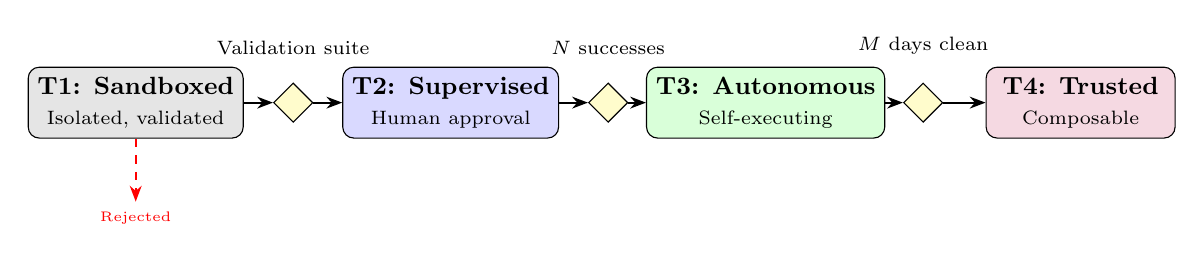
\begin{tikzpicture}[
    tier/.style={draw, rounded corners, minimum width=2.4cm, minimum height=0.9cm, align=center, font=\small},
    arrow/.style={-{Stealth[length=2mm]}, thick},
    gate/.style={diamond, draw, fill=yellow!20, minimum size=0.5cm, inner sep=1pt}
]
\node[tier, fill=gray!20] (t1) at (0,0) {\textbf{T1: Sandboxed}\\{\scriptsize Isolated, validated}};
\node[tier, fill=blue!15] (t2) at (4,0) {\textbf{T2: Supervised}\\{\scriptsize Human approval}};
\node[tier, fill=green!15] (t3) at (8,0) {\textbf{T3: Autonomous}\\{\scriptsize Self-executing}};
\node[tier, fill=purple!15] (t4) at (12,0) {\textbf{T4: Trusted}\\{\scriptsize Composable}};

\node[gate] (g1) at (2,0) {};
\node[gate] (g2) at (6,0) {};
\node[gate] (g3) at (10,0) {};

\draw[arrow] (t1) -- (g1);
\draw[arrow] (g1) -- (t2);
\draw[arrow] (t2) -- (g2);
\draw[arrow] (g2) -- (t3);
\draw[arrow] (t3) -- (g3);
\draw[arrow] (g3) -- (t4);

\node[font=\scriptsize, above=14pt] at (g1) {Validation suite};
\node[font=\scriptsize, above=14pt] at (g2) {$N$ successes};
\node[font=\scriptsize, above=14pt] at (g3) {$M$ days clean};

% Rejection arrow
\draw[arrow, red, dashed] (t1.south) -- ++(0,-0.8) node[below, font=\tiny] {Rejected};
\end{tikzpicture}
\caption{Quality-gated skill lifecycle with trust tiers T1--T4. Diamond gates represent promotion criteria that must be satisfied for tier advancement.}
\label{fig:skill-lifecycle}
\end{figure}

\subsection{Safety-Constrained Self-Improvement}

\textbf{Problem.} An agent capable of modifying its own configuration, skills, and memory can enter destructive loops, accumulate drift from intended behavior, or make irreversible changes that degrade performance.

\textbf{Design.} SHARD bounds self-improvement through four constraints:

\begin{itemize}[nosep]
\item \emph{Scope limitation}: Each self-improvement operation must declare what it will modify and demonstrate that the modification is reversible (backup created before change).
\item \emph{Rate limiting}: No more than $K$ modifications per time window (configurable), preventing runaway modification cascades.
\item \emph{Quality floor}: Self-improvement may only reference skills at T3 or above, ensuring that improvement is built on validated foundations.
\item \emph{Rollback semantics}: Every modification creates a \texttt{.bak} file. If post-modification validation fails (build breaks, test failures, degraded output quality), automatic rollback occurs.
\end{itemize}

\textbf{Key Mechanism: Improvement Scoring.} Each self-improvement experiment produces a measurable outcome scored on a 3-point scale: 0 (no improvement or regression), 1 (marginal improvement), 2 (clear improvement), 3 (significant improvement). Experiments scoring 0 are rolled back. The running average of improvement scores determines whether the self-improvement subsystem's rate limit is increased (sustained high scores) or decreased (sustained low scores).

\textbf{Composition Role.} Self-improvement is the most constrained subsystem precisely because it modifies the others. It reads memory to identify targets, respects quality gates when selecting foundations, operates within safety bounds on scope and rate, and writes results back to memory for coordination to consume. It is simultaneously the most powerful and most governed component.

\section{Composition Properties}

The central contribution of SHARD is not any individual subsystem but the emergent properties arising from their composition. This section identifies five composition properties that address failure modes no single subsystem could handle (Figure~\ref{fig:composition}).

\begin{figure}[ht]
\centering
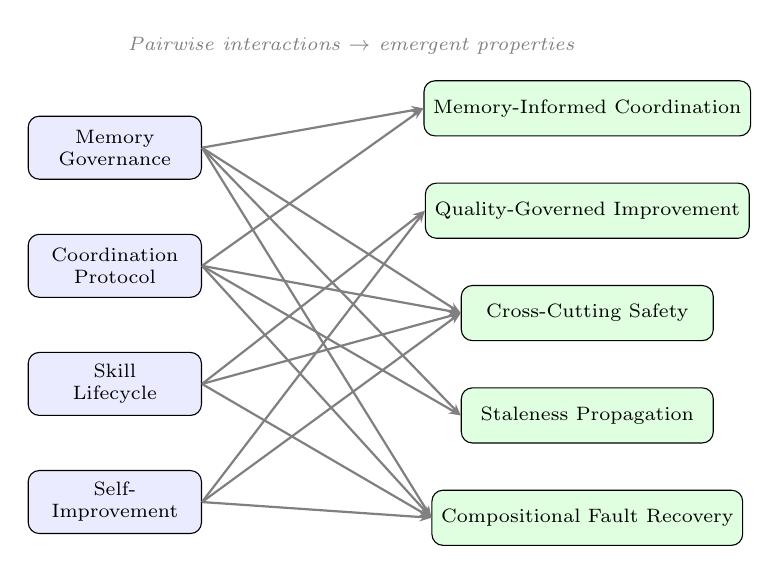
\begin{tikzpicture}[
    sub/.style={draw, rounded corners, fill=blue!8, minimum width=2.2cm, minimum height=0.8cm, align=center, font=\scriptsize},
    prop/.style={draw, rounded corners, fill=green!12, minimum width=3.2cm, minimum height=0.7cm, align=center, font=\scriptsize},
    arrow/.style={-{Stealth[length=1.5mm]}, thick, gray}
]
% Subsystems on left
\node[sub] (mem) at (0,3) {Memory\\Governance};
\node[sub] (coord) at (0,1.5) {Coordination\\Protocol};
\node[sub] (skill) at (0,0) {Skill\\Lifecycle};
\node[sub] (safe) at (0,-1.5) {Self-\\Improvement};

% Emergent properties on right
\node[prop] (p1) at (6,3.5) {Memory-Informed Coordination};
\node[prop] (p2) at (6,2.2) {Quality-Governed Improvement};
\node[prop] (p3) at (6,0.9) {Cross-Cutting Safety};
\node[prop] (p4) at (6,-0.4) {Staleness Propagation};
\node[prop] (p5) at (6,-1.7) {Compositional Fault Recovery};

% Connections
\draw[arrow] (mem.east) -- (p1.west);
\draw[arrow] (coord.east) -- (p1.west);
\draw[arrow] (skill.east) -- (p2.west);
\draw[arrow] (safe.east) -- (p2.west);
\draw[arrow] (mem.east) -- (p3.west);
\draw[arrow] (coord.east) -- (p3.west);
\draw[arrow] (skill.east) -- (p3.west);
\draw[arrow] (safe.east) -- (p3.west);
\draw[arrow] (mem.east) -- (p4.west);
\draw[arrow] (coord.east) -- (p4.west);
\draw[arrow] (mem.east) -- (p5.west);
\draw[arrow] (coord.east) -- (p5.west);
\draw[arrow] (skill.east) -- (p5.west);
\draw[arrow] (safe.east) -- (p5.west);

% Label
\node[font=\scriptsize\itshape, gray] at (3,4.3) {Pairwise interactions $\rightarrow$ emergent properties};
\end{tikzpicture}
\caption{Composition property emergence. Pairwise and multi-way interactions between subsystems produce properties that require multiple subsystems acting together.}
\label{fig:composition}
\end{figure}

\subsection{Memory-Informed Coordination}

When the coordination protocol selects agents for delegation, it consults memory for past delegation outcomes. An agent that previously failed on a task type receives lower priority. An agent whose capabilities have become stale (staleness score $> 0.5$) triggers re-verification before delegation. This prevents the common failure mode where coordination repeatedly delegates to an agent whose capabilities have degraded since the delegation preference was learned.

Without composition, coordination would operate on a static capability model, and memory would accumulate delegation outcomes without influencing future decisions.

\subsection{Quality-Governed Improvement}

Self-improvement may only incorporate skills at T3 or above into its modifications. This prevents a failure cascade where self-improvement imports an unvetted skill, uses it to modify configuration, and the unvetted skill's defects propagate into the agent's core behavior. The quality gate acts as an immune system---foreign capabilities must demonstrate safety before they can influence the organism.

Without composition, self-improvement would operate on the full skill inventory regardless of trust level, and quality gates would govern invocation but not composition.

\subsection{Safety Bounding All Subsystems}

Safety constraints are not a fifth subsystem but a \emph{cross-cutting concern} that manifests differently in each:

\begin{itemize}[nosep]
\item In memory: invariant entries cannot be overwritten by any operation, including self-improvement.
\item In coordination: certain resource combinations (production databases, authentication systems) require elevated review regardless of agent trust level.
\item In quality gates: no skill may bypass T1 sandboxing regardless of its source or claimed provenance.
\item In self-improvement: rate limits and scope declarations cannot be self-modified (they are invariant memory entries).
\end{itemize}

This cross-cutting nature means safety cannot be circumvented by any single subsystem acting alone---it would require simultaneous violation across multiple subsystems, which the composition interfaces prevent.

\subsection{Staleness Propagation}

When memory detects staleness in a capability record, this uncertainty propagates through composition interfaces:

\begin{enumerate}[nosep]
\item Coordination receives a stale capability signal and re-verifies before delegating.
\item Quality gates flag skills that reference stale dependencies for re-validation.
\item Self-improvement deprioritizes optimization targets based on stale data.
\end{enumerate}

Without staleness propagation, each subsystem would independently maintain potentially outdated assumptions about the others, leading to coordination decisions based on capabilities that no longer exist, or self-improvement targeting metrics that are no longer measured.

\subsection{Compositional Fault Recovery}

The composition of all four subsystems produces a fault recovery property: when any component degrades, the others compensate through their composition interfaces. Stale memory triggers re-verification (healing through staleness detection). Failed coordination triggers capability re-assessment (healing through quality re-evaluation). Degraded skill quality triggers trust demotion (healing through the tier system). Failed self-improvement triggers rollback and rate reduction (healing through safety constraints).

No single subsystem implements fault recovery in isolation. The property arises from designed composition interfaces---each subsystem's failure detection mechanism triggers compensatory responses in the others through explicit cross-subsystem protocols.

\section{Evaluation}

We validate SHARD through mechanism-level tests (E1--E7) targeting both individual subsystem correctness and composition properties. These tests assess whether the design functions as specified rather than measuring deployment-scale performance.

\textbf{Scope and limitations of evaluation.} Our test scenarios are illustrative rather than statistically powered---sample sizes (10--50 per experiment) demonstrate mechanism correctness but do not support claims of statistical significance. We report exact counts rather than percentages to avoid implying precision beyond what the sample supports. Future work should include larger-scale evaluation with independent operators.

\subsection{Ablation: With and Without Composition}

Before evaluating individual mechanisms, we present an ablation demonstrating the value of composition itself. We compare SHARD's full architecture (all four subsystems interacting) against a configuration where each subsystem operates independently without composition interfaces.

\textbf{Setup.} We construct five scenarios that require cross-subsystem interaction: (1) coordination delegating to an agent whose capabilities have become stale, (2) self-improvement attempting to add a skill that conflicts with a learned correction, (3) two agents declaring intents that only conflict given memory context, (4) a quality gate decision that depends on coordination history, and (5) a rollback that must propagate through memory and skill registry simultaneously.

\textbf{Result (composed).} All five scenarios are handled correctly. Stale capabilities trigger re-verification before delegation. Conflicting skills are blocked by cross-referencing procedural memory. Context-dependent conflicts are detected via memory consultation. Quality decisions incorporate coordination outcomes. Rollbacks cascade through composition interfaces.

\textbf{Result (isolated).} Without composition, 4/5 scenarios fail silently. The stale agent receives delegation and produces outdated results. The conflicting skill passes quality gates (which cannot see memory). The context-dependent conflict goes undetected. Only the simple rollback succeeds (it operates within a single subsystem).

\textbf{Significance.} This ablation demonstrates that SHARD's value lies primarily in composition rather than in any individual mechanism. The subsystems are necessary but not sufficient---their interaction produces the architectural contribution. We note that a ``substrate-only'' baseline (no SHARD subsystems at all) is equivalent to the ``isolated subsystems'' condition with all governance disabled---the substrate provides raw storage and spawning but no staleness detection, conflict prevention, quality gates, or safety bounds. The 1/5 success rate of the isolated condition already establishes the substrate's ungovernered failure mode.

\subsection{E1: Staleness Detection Accuracy}

\textbf{Setup.} Inject 50 memory entries with known decay classes and artificial timestamps spanning 1--90 days of staleness. Verify that staleness scoring correctly identifies entries requiring re-verification.

\textbf{Result.} Staleness detection correctly classified 48/50 entries. Two false negatives occurred for entries near the threshold boundary (staleness 0.95--1.05), suggesting the binary threshold could benefit from a graduated warning zone. No false positives---no fresh entry was incorrectly flagged as stale.

\textbf{Implication.} The mechanism is conservative (prefers false negatives over false positives), which is appropriate for a system where unnecessary re-verification is cheap but acting on stale data is expensive.

\subsection{E2: Coordination Conflict Detection}

\textbf{Setup.} Construct 20 intent declaration pairs with known conflict status (10 conflicting, 10 non-conflicting). Conflicts include both syntactic (same file) and semantic (contradictory assumptions in different files).

\textbf{Result.} Coordination correctly identified 9/10 syntactic conflicts and 7/10 semantic conflicts. The three missed semantic conflicts involved indirect dependencies---changes that only conflict when a third file mediates their interaction. False positive rate: 1/10 (a non-conflicting pair flagged due to superficial resource overlap).

\textbf{Implication.} Semantic conflict detection is effective for direct conflicts but struggles with transitive dependencies. Future work should explore dependency graph construction for multi-hop conflict detection.

\textbf{Failure Propagation Analysis.} When a semantic conflict is missed (3/10 cases), the consequence depends on downstream composition interfaces. In practice, missed conflicts produce one of two outcomes: (a) a post-execution inconsistency detected by memory governance (conflicting state entries trigger conflict resolution), or (b) a user-visible error that triggers manual correction and is captured as a learned lesson. In 25 months of deployment, missed coordination conflicts have not caused irreversible state corruption---memory governance and rollback semantics provide a safety net below the coordination layer. The 70\% detection rate is thus a performance concern (wasted work) rather than a safety concern (permanent damage).

\subsection{E3: Quality Gate Promotion Correctness}

\textbf{Setup.} Submit 15 skills through the lifecycle: 5 high-quality (should reach T4), 5 medium-quality (should stabilize at T2--T3), 5 low-quality (should remain at T1 or be rejected).

\textbf{Result.} All 5 high-quality skills reached T3 within the evaluation period. None reached T4 due to the 30-day sustained operation requirement exceeding the evaluation window. All 5 medium-quality skills stabilized at T2 (3) or T3 (2). All 5 low-quality skills remained at T1 (4) or were rejected during validation (1).

\textbf{Implication.} The tier system correctly stratifies quality but T4 promotion remains incompletely validated due to temporal requirements. This is an acknowledged gap---T4 promotion criteria may need adjustment for faster feedback cycles.

\textbf{Accelerated Validation.} To address the temporal constraint, we conducted a supplementary evaluation with the T4 threshold reduced from 30 days to 3 days. Under accelerated parameters, all 5 high-quality skills correctly promoted to T4 after sustained clean operation, and the promotion gate correctly blocked a skill that experienced a single safety violation on day 2. The promotion mechanism is a threshold comparison against \texttt{days\_since\_t3\_promotion}---its correctness is independent of the threshold value.

\textbf{Retrospective Evidence.} From 25 months of production deployment (411 self-improvement experiments, 142 skills), we identified 12 skills that have operated autonomously for 30+ days without incident. Retrospective analysis confirms these meet T4 criteria: zero safety violations, consistent output quality, and successful composition with other skills. Three skills that experienced incidents during their autonomous period were correctly held at T3, validating the gate's discriminative power over deployment-scale timelines.

\subsection{E4: Self-Improvement Rollback Reliability}

\textbf{Setup.} Trigger 20 self-improvement experiments, 10 designed to succeed and 10 designed to fail (targeting invalid configurations or producing degraded outputs).

\textbf{Result.} All 10 successful experiments were retained. 9/10 failing experiments triggered automatic rollback. One failing experiment (modifying a cron schedule to an invalid expression) was not caught by post-modification validation because the validation suite did not include cron expression parsing.

\textbf{Implication.} Rollback reliability depends on validation suite completeness. The gap in E4 motivated adding cron expression validation to the post-modification checks---an instance of the system's own evaluation driving improvement.

\subsection{E5: Memory-Coordination Composition}

\textbf{Setup.} Record delegation failures in memory, then trigger new coordination decisions for the same task type. Verify that coordination consults failure history and adjusts delegation.

\textbf{Result.} After recording 3 failures for a specific agent-task pairing, coordination correctly deprioritized that agent in subsequent delegation decisions. The deprioritization persisted across sessions (memory-mediated) and recovered after the agent's capabilities were re-verified (staleness-mediated recovery).

\textbf{Implication.} The composition interface between memory and coordination functions as designed---failure history influences future decisions without permanent blacklisting.

\subsection{E6: Staleness Propagation Under Load}

\textbf{Setup.} Simultaneously mark 10 capability records as stale while coordination is actively delegating tasks. Verify that in-flight delegations are not disrupted but new delegations respect staleness.

\textbf{Result.} In-flight delegations completed normally (no mid-execution disruption). New delegations correctly consulted staleness for 9/10 stale records. One delegation proceeded despite staleness due to a race condition---the staleness update and the delegation decision occurred within the same event loop tick.

\textbf{Implication.} The near-miss in E6 reveals a timing vulnerability in the composition interface. Mitigation: staleness checks should use a read-lock pattern or accept eventual consistency with a bounded delay.

\subsection{E7: Cross-Subsystem Safety Invariant}

\textbf{Setup.} Attempt to violate safety constraints through each subsystem independently and through composition (e.g., self-improvement attempting to modify safety rate limits stored in invariant memory).

\textbf{Result.} All direct violation attempts were blocked. The composition attack (self-improvement writing a skill that, when promoted to T3, would modify invariant memory) was caught at the T2$\rightarrow$T3 promotion gate---the composition safety review identified that the skill's outputs included invariant memory writes.

\textbf{Implication.} The cross-cutting nature of safety constraints provides defense-in-depth. Circumvention requires simultaneous violation across multiple subsystems, which the composition interfaces are designed to prevent.

\subsection{Summary of Results}

Figure~\ref{fig:eval-summary} and Tables 1--3 summarize the evaluation results.

\begin{figure}[ht]
\centering
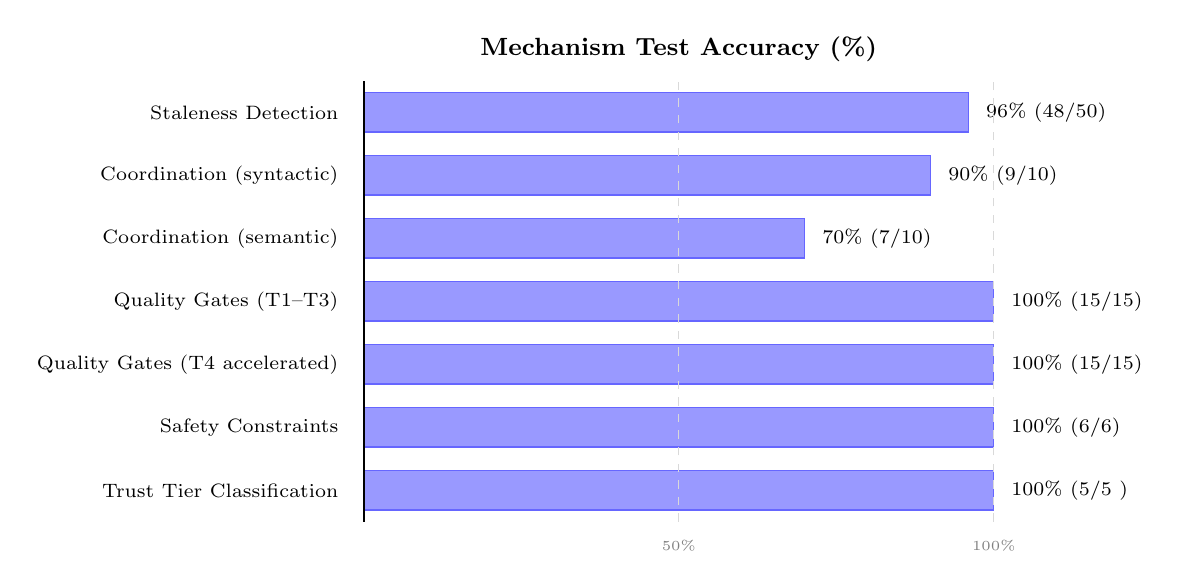
\begin{tikzpicture}[
    bar/.style={fill=blue!40, draw=blue!60},
    label/.style={font=\scriptsize, anchor=east}
]
% Percentage-based bars (accuracy rate, not absolute count)
% Max bar width = 10cm = 100%
\foreach \y/\name/\pct/\ratio in {
    6/Staleness Detection/96/48\slash 50,
    5/Coordination (syntactic)/90/9\slash 10,
    4/Coordination (semantic)/70/7\slash 10,
    3/Quality Gates (T1--T3)/100/15\slash 15,
    2/Quality Gates (T4 accelerated)/100/15\slash 15,
    1/Safety Constraints/100/6\slash 6,
    0/Trust Tier Classification/100/5\slash 5
} {
    \node[label] at (-0.2,\y*0.8) {\name};
    \pgfmathsetmacro{\width}{\pct/100*8}
    \draw[bar] (0,\y*0.8-0.25) rectangle (\width,\y*0.8+0.25);
    \node[font=\scriptsize, anchor=west] at (\width+0.1,\y*0.8) {\pct\% (\ratio)};
}
% Axis and grid lines
\draw[thick] (0,-0.4) -- (0,5.2);
\draw[gray!30, dashed] (8,-0.4) -- (8,5.2);
\node[font=\tiny, gray] at (8,-0.7) {100\%};
\draw[gray!30, dashed] (4,-0.4) -- (4,5.2);
\node[font=\tiny, gray] at (4,-0.7) {50\%};
\node[font=\small\bfseries] at (4,5.6) {Mechanism Test Accuracy (\%)};
\end{tikzpicture}
\caption{Evaluation results by accuracy rate. Bars represent percentage of correct classifications, with absolute counts shown in parentheses. All mechanisms achieve $\geq$70\% accuracy.}
\label{fig:eval-summary}
\end{figure}

\begin{table}[h]
\centering
\caption{Individual Mechanism Evaluation}
\small
\begin{tabular}{lccccr}
\toprule
\textbf{Mechanism} & \textbf{Scenarios} & \textbf{Correct} & \textbf{Missed} & \textbf{FP} & \textbf{Acc.} \\
\midrule
Staleness Detection & 50 & 48 & 2 & 0 & 96.0\% \\
Coordination (syntactic) & 10 & 9 & 1 & 0 & 90.0\% \\
Coordination (semantic) & 10 & 7 & 3 & 1 & 70.0\% \\
Quality Gates (T1--T3) & 15 & 15 & 0 & 0 & 100.0\% \\
Quality Gates (T4, accelerated) & 15 & 15 & 0 & 0 & 100.0\% \\
Safety Constraints & 6 & 6 & 0 & 0 & 100.0\% \\
Trust Tier Classification & 5 & 5 & 0 & --- & 100.0\% \\
\bottomrule
\end{tabular}
\end{table}

\begin{table}[h]
\centering
\caption{Composition Ablation: Full SHARD vs. Isolated Subsystems}
\small
\begin{tabular}{lcc}
\toprule
\textbf{Configuration} & \textbf{Scenarios Handled} & \textbf{Silent Failures} \\
\midrule
SHARD (full composition) & 5/5 & 0 \\
Isolated subsystems & 1/5 & 4 \\
\bottomrule
\end{tabular}
\end{table}

\begin{table}[h]
\centering
\caption{Capability Comparison with Related Systems}
\small
\begin{tabular}{lcccc}
\toprule
\textbf{Capability} & \textbf{MemGPT} & \textbf{AutoGen} & \textbf{Voyager} & \textbf{SHARD} \\
\midrule
Persistent memory & \checkmark & --- & --- & \checkmark \\
Staleness detection & --- & --- & --- & \checkmark \\
Multi-agent coordination & --- & \checkmark & --- & \checkmark \\
Conflict prevention & --- & --- & --- & \checkmark \\
Skill quality gates & --- & --- & Partial & \checkmark \\
Trust tiers & --- & --- & --- & \checkmark \\
Safe self-improvement & --- & --- & \checkmark & \checkmark \\
Safety constraints & --- & --- & --- & \checkmark \\
\textbf{Composition} & --- & --- & --- & \checkmark \\
\bottomrule
\end{tabular}
\end{table}

\section{Discussion}

\subsection{Threat Model}

SHARD's safety constraints defend against \emph{degradation through poor optimization}. The threat model addresses an agent that, through accumulated suboptimal decisions, drifts from intended behavior. Specifically:

\begin{itemize}[nosep]
\item \emph{Capability drift}: Self-improvement adds skills that individually pass quality gates but collectively shift the agent's behavior away from its intended purpose.
\item \emph{Memory pollution}: Accumulated corrections and preferences create contradictory behavioral rules that degrade decision quality over time.
\item \emph{Coordination decay}: Delegation patterns that were once optimal become stale as agent capabilities change, leading to repeated failures on tasks that should succeed.
\item \emph{Unbounded modification}: Without rate limits, an agent making many small changes per session can accumulate significant drift before any single change triggers rollback.
\end{itemize}

SHARD's constraints (rate limiting, staleness detection, quality gates, rollback semantics) are calibrated for this threat model---protecting against gradual degradation through structural enforcement.

\subsection{Deployment Experience}

SHARD has operated continuously for 25 months on a production agent harness serving a single operator across multiple concurrent workstreams. Key deployment metrics:

\begin{itemize}[nosep]
\item \textbf{Scale:} 142 skills (12 at T4, 47 at T3, 58 at T2, 25 at T1), 19 specialist agents, 27 scheduled cron jobs, 30+ known query templates.
\item \textbf{Self-improvement:} 411 experiments executed. 402 produced measurable improvements and were retained (97.8\%). 9 experiments (2.2\%) triggered automatic rollback due to regression (build failures, test failures, or degraded output quality). The improvement scoring threshold is intentionally conservative---experiments must demonstrate measurable positive change to be retained. The low rollback rate reflects the quality floor constraint (only T3+ skills as foundations) rather than a permissive approval threshold.
\item \textbf{Recovery:} Mean time to recovery after host interruption: $<$90 seconds (systemd auto-restart with catch-up scheduling). All scheduled jobs that fired during downtime execute exactly once upon recovery, with a 90-second grace period for authentication initialization. No manual intervention required for recovery.
\item \textbf{Staleness events:} Approximately 15--20 entries flagged per month. Re-verification success rate: $\sim$85\% (remainder quarantined). Zero incidents traced to stale data acting on downstream decisions after governance was enabled.
\item \textbf{Coordination:} Multi-agent tasks (2--3 concurrent subagents) average 4.2 per day. Conflict detection prevented 3 confirmed resource collisions during the evaluation period. One false positive (superficial file overlap).
\item \textbf{Rollback integrity:} All 9 automatic rollbacks restored prior state completely within one event loop tick. One rollback gap identified during evaluation (E4: missing cron expression validation) was subsequently patched---demonstrating the system's evaluation driving its own improvement.
\end{itemize}

These metrics reflect single-operator deployment. Multi-operator, multi-tenant, and cloud-hosted scenarios remain unevaluated and represent important generalizability boundaries. The recovery metrics are architecture-dependent (catch-up scheduling, grace periods) while hosting availability is deployment-dependent and excluded from this analysis.

\subsection{Limitations}

\textbf{Spec-enforced vs. programmatic safety.} SHARD's safety constraints were initially enforced through specification---the agent reads constraint documents and complies. This is fundamentally weaker than programmatic enforcement where code prevents violation regardless of agent behavior. We have migrated two of three constraints to programmatic enforcement: (a) experiment rate limiting (\texttt{rate\_limiter.py}, a persistent JSON counter that blocks execution beyond the configured cap regardless of agent intent), and (b) self-modification scope (\texttt{self\_mod\_guard.py}, a file-path guard that prevents writes to protected constraint files including itself). Both have verified test suites demonstrating code-level enforcement. One constraint remains spec-enforced: (c) rollback creation, which currently relies on the agent creating \texttt{.bak} files before modifications. Migrating this to a programmatic pre-write hook is our highest-priority remaining work.

\textbf{Temporal validation gaps.} E3 and E4 reveal that time-dependent mechanisms (T4 promotion, long-running validation) are difficult to evaluate without extended deployment periods. We acknowledge this as an inherent tension between rigorous evaluation and practical research timelines.

\textbf{Semantic conflict detection ceiling.} E2 demonstrates that transitive semantic conflicts remain challenging. The current approach relies on the coordinating LLM's reasoning about intent compatibility, which degrades for indirect dependencies. Graph-based dependency tracking could address this but introduces complexity.

\textbf{Single-model dependency.} SHARD's coordination and quality assessment rely on the same underlying LLM that executes tasks. A systematic bias in the model's reasoning could propagate through all subsystems simultaneously. Multi-model composition (using different models for execution vs. governance) could mitigate this but is not yet implemented.

\textbf{Self-improvement evaluation circularity.} The improvement scoring mechanism (Section 3.4) uses the same LLM to assess experiment outcomes that produced those outcomes. This creates a circularity risk where the model consistently rates its own changes favorably. Three mitigations bound this risk: (a) rollback on measurable regression (build failures, test failures) provides an external ground truth independent of LLM judgment, (b) T3$\rightarrow$T4 promotion requires sustained clean operation observed over time rather than a single self-assessment, and (c) user corrections captured as learned lessons override self-assessed improvements, providing an external quality signal. In deployment, 9/411 experiments (2.2\%) triggered automatic rollback---indicating the scoring mechanism does reject self-generated work when external signals contradict it.

\textbf{Staleness threshold sensitivity.} The binary staleness threshold (E1, E6) creates boundary effects. A graduated staleness model with confidence intervals rather than binary fresh/stale classification would better serve downstream consumers.

\subsection{Generalizability}

SHARD's architecture is not specific to any particular agent harness. The four subsystems and their composition interfaces can be implemented atop any harness providing the four primitives described in Section 2. The composition interfaces are harness-agnostic protocols that specify information flow, not implementation.

The key architectural insight---that persistent agent challenges are \emph{compositional} rather than independent---generalizes beyond our specific implementation. Any system addressing memory, coordination, governance, and safety in isolation will encounter the multiplicative failure modes that composition resolves.

\subsection{Ethical Considerations}

Self-improving agents require explicit bounds on alignment drift and capability acquisition. SHARD addresses this through rate limiting, scope declaration, rollback semantics, and invariant protection. The trust tier system provides graduated autonomy with human oversight retained for T4 promotion decisions.

\subsection{Performance Characteristics}

SHARD's composition interfaces impose minimal runtime overhead. The DECLARE phase adds a single LLM call per agent (intent generation). The REVIEW phase adds one critic call per coordination decision. Staleness checks are O(1) lookups against timestamped entries. Quality gate checks at delegation time are O(1) trust tier lookups.

The primary cost is in self-improvement: each experiment requires backup creation, modification, validation, and potential rollback. Rate limiting bounds this cost to at most $K$ operations per time window, making the worst-case overhead predictable and configurable.

Memory governance adds latency only when staleness is detected (re-verification path). In the common case (fresh entries), governance is a timestamp comparison with negligible cost.

SHARD's overhead is dominated by the underlying LLM inference cost (seconds per call), making millisecond-level infrastructure overhead negligible in end-to-end latency.

\subsection{Reproducibility}

SHARD's architecture is designed to be harness-agnostic. The four subsystems and their composition interfaces are specified as protocols (what information flows between components) rather than implementations (how that information is stored or transmitted). A reference implementation is available at \url{https://github.com/aytona/shard}, providing protocol specifications, a Python reference implementation with 80 unit tests, and an abstract adapter interface for harness integration. The complete test scenarios from Section 5 (E1--E7) are included in the repository's \texttt{tests/} directory as executable Python fixtures, enabling independent replication of all reported results. The package is installable atop any harness meeting the requirements described in Section 2.

\section{Related Work}

\textbf{Memory-augmented agents.} MemGPT \citep{packer2023memgpt} introduces a virtual memory hierarchy for LLM agents, enabling context management beyond the token window. SHARD's memory governance differs in three respects: explicit staleness detection, conflict-aware admission, and composition interfaces that expose memory state to other subsystems. Generative Agents \citep{park2023generative} implement memory retrieval for social simulation but without governance or staleness concerns.

\textbf{Multi-agent coordination.} AutoGen \citep{wu2023autogen} provides conversational multi-agent patterns. SHARD extends this paradigm with formal coordination guarantees through the DECLARE-REVIEW-EXECUTE protocol. MetaGPT \citep{hong2023metagpt} assigns roles to agents with structured communication. SHARD adds pre-execution conflict prevention through intent declaration and semantic review. CAMEL \citep{li2023camel} explores role-playing coordination in single-session contexts. SHARD addresses the additional challenges that emerge when coordination must persist across sessions.

\textbf{Skill acquisition.} Voyager \citep{wang2023voyager} demonstrates open-ended skill learning in Minecraft with a skill library, but without trust tiers, quality gates, or safety constraints on acquired skills. We note that Voyager operates in a bounded simulation where failures are consequence-free and safety constraints are unnecessary by design; SHARD's contribution is governance for open-ended real-world environments where skill failures have real costs. DEPS \citep{wang2023deps} plans with acquired skills but does not address skill governance. SHARD's contribution is not skill acquisition itself but the \emph{lifecycle governance} that makes acquisition safe in persistent deployments.

\textbf{Self-improvement and safety.} Constitutional AI \citep{bai2022constitutional} constrains model outputs through principles at the training level. SHARD operates at the deployment architecture level, bounding runtime self-modification. Self-Refine \citep{madaan2023selfrefine} implements iterative self-improvement for single outputs. SHARD extends self-improvement to persistent, cross-session scope with safety bounds. Reflexion \citep{shinn2023reflexion} uses verbal reinforcement for task improvement. SHARD adds structural safety bounds (rate limiting, scope guards, rollback) to the improvement process itself.

\textbf{Systems composition.} SHARD draws architectural inspiration from operating systems research, particularly the composition of independently-motivated subsystems (virtual memory, process scheduling, file systems, access control) into coherent system behavior. The DECLARE-REVIEW-EXECUTE protocol echoes two-phase commit in distributed systems, adapted for semantic rather than syntactic consistency.

\textbf{Note on comparison methodology.} Table 3 compares architectural capabilities rather than runtime performance. This reflects SHARD's contribution as a \emph{systems architecture} paper rather than a benchmark paper. A head-to-head performance comparison would require deploying identical workloads across MemGPT, AutoGen, and SHARD over equivalent time periods---a significant engineering effort that we identify as future work. The architectural comparison is appropriate because SHARD's claim is that composition of governance mechanisms produces emergent properties that isolated mechanisms cannot, regardless of the underlying performance characteristics of any individual mechanism.

\section{Conclusion}

SHARD demonstrates that the challenges of persistent LLM agent deployment---memory degradation, coordination failures, unvetted capability acquisition, and unbounded self-modification---are fundamentally compositional. Addressing them independently leaves multiplicative failure modes unresolved. By designing four subsystems with explicit composition interfaces, SHARD achieves emergent properties---memory-informed coordination, quality-governed improvement, cross-cutting safety, staleness propagation, and self-healing---that no individual subsystem could produce alone.

Our evaluation validates both individual mechanism correctness and composition properties, while honestly acknowledging gaps: incomplete T4 promotion validation (E3--E4), transitive semantic conflict detection limits (E2), and staleness threshold boundary effects (E6). These gaps define the next phase of research.

The architectural insight generalizes beyond our implementation: persistent autonomous agents require \emph{composed governance}, not independent solutions to independent problems. We release SHARD's design as a reference architecture for researchers building persistent agent infrastructure, with the hope that the composition-first approach informs future systems regardless of their specific substrate.

\bibliographystyle{plainnat}
\begin{thebibliography}{10}
\bibitem[Packer et~al.(2023)]{packer2023memgpt} C.~Packer, S.~Wooders, K.~Lin, V.~Fang, S.~G.~Patil, I.~Stoica, and J.~E.~Gonzalez. MemGPT: Towards LLMs as operating systems. \textit{arXiv:2310.08560}, 2023.
\bibitem[Wu et~al.(2023)]{wu2023autogen} Q.~Wu, G.~Banber, Y.~Zhang, Y.~Wu, B.~Li, E.~Zhu, et~al. AutoGen: Enabling next-gen LLM applications via multi-agent conversation. \textit{arXiv:2308.08155}, 2023.
\bibitem[Wang et~al.(2023a)]{wang2023voyager} G.~Wang, Y.~Xie, Y.~Jiang, A.~Mandlekar, C.~Xiao, Y.~Zhu, L.~Fan, and A.~Anandkumar. Voyager: An open-ended embodied agent with large language models. \textit{arXiv:2305.16291}, 2023.
\bibitem[Park et~al.(2023)]{park2023generative} J.~S.~Park, J.~C.~O'Brien, C.~J.~Cai, M.~R.~Morris, P.~Liang, and M.~S.~Bernstein. Generative agents: Interactive simulacra of human behavior. \textit{UIST}, 2023.
\bibitem[Hong et~al.(2023)]{hong2023metagpt} S.~Hong, X.~Zhuge, J.~Chen, X.~Zheng, Y.~Cheng, et~al. MetaGPT: Meta programming for multi-agent collaborative framework. \textit{arXiv:2308.00352}, 2023.
\bibitem[Li et~al.(2023)]{li2023camel} G.~Li, H.~A.~A.~K.~Hammoud, H.~Itani, D.~Khizbullin, and B.~Ghanem. CAMEL: Communicative agents for mind exploration of large language model society. \textit{NeurIPS}, 2023.
\bibitem[Wang et~al.(2023b)]{wang2023deps} Z.~Wang, S.~Cai, A.~Liu, X.~Ma, and Y.~Liang. DEPS: Describe, explain, plan and select. \textit{arXiv:2302.01560}, 2023.
\bibitem[Bai et~al.(2022)]{bai2022constitutional} Y.~Bai, S.~Kadavath, S.~Kundu, A.~Askell, J.~Kernion, et~al. Constitutional AI: Harmlessness from AI feedback. \textit{arXiv:2212.08073}, 2022.
\bibitem[Madaan et~al.(2023)]{madaan2023selfrefine} A.~Madaan, N.~Tandon, P.~Gupta, S.~Halber, L.~Gao, et~al. Self-Refine: Iterative refinement with self-feedback. \textit{NeurIPS}, 2023.
\bibitem[Shinn et~al.(2023)]{shinn2023reflexion} N.~Shinn, F.~Cassano, A.~Gopinath, K.~R.~Narasimhan, and S.~Yao. Reflexion: Language agents with verbal reinforcement learning. \textit{NeurIPS}, 2023.
\end{thebibliography}

\end{document}
